\documentclass[11pt, a4paper]{article}
\usepackage[ukrainian]{babel}
\usepackage[a4paper, top=2.5cm, bottom=2.5cm, left=2cm, right=2cm]{geometry}
\usepackage{fontspec}
\usepackage{amsmath}
\usepackage{amssymb}
\usepackage{enumitem}
\usepackage{graphicx}

% Налаштування шрифтів для коректного відображення української мови в LaTeX
% (Helvetica — системний шрифт macOS; за наявності Noto Sans можна замінити)
\babelfont{rm}{Helvetica}
\babelfont[ukrainian]{rm}{Helvetica}
\setlist[itemize]{label=-}

\title{\textbf{Лекція 8. Дослідження особливих точок та періодичних розв'язків \\ (Приклади)}}
\author{}
\date{2026р}

\begin{document}

\maketitle

\section*{Приклад 1}
Розглядається система:
\begin{gather*}
\begin{cases}
\dot{x} = P(x,y) = y \\
\dot{y} = Q(x,y) = 2(1 - x^2)y
\end{cases}
\end{gather*}

Пошук особливих точок (станів рівноваги):
$$\begin{cases} y = 0 \\ 2(1 - x^2)y = 0 \end{cases}$$

Оскільки при $y = 0$ вся вісь $OX$ складається з розв'язків ($x \in \mathbb{R}$, особливі точки), система не має \textbf{ізольованих} станів рівноваги.

---

\section*{Приклад 2}
Розглядається система з $\epsilon$-параметрами:
\begin{gather*}
\begin{cases}
\dot{x} = y \\
\dot{y} = x + x^2 - (\epsilon_1 + \epsilon_2 x)y
\end{cases}
\end{gather*}

$1^{\circ}$ Особлива точка $O(0,0)$. \\
$2^{\circ}$ Особлива точка $A(-1, 0)$.

Знайдемо частинні похідні для лінеаризації:
$$P_x = 0, \quad P_y = 1, \quad Q_x = 1 + 2x, \quad Q_y = -(\epsilon_1 + \epsilon_2 x)$$

Для $1^{\circ}$ особливої точки $O(0,0)$:
$$P_x Q_y - P_y Q_x = 0 - 1 \cdot 1 = -1 < 0 \implies O(0,0) \text{ -- сідло}$$

Для $2^{\circ}$ особливої точки $A(-1,0)$: \\
Характеристичне рівняння:
$$\lambda^2 + (\epsilon_1 - \epsilon_2)\lambda + 1 = 0 \implies \lambda_{1,2} = \frac{-(\epsilon_1 - \epsilon_2) \pm \sqrt{(\epsilon_1 - \epsilon_2)^2 - 4}}{2}$$

Характер спокою (стійкості) стану рівноваги $A(-1,0)$ залежно від параметрів:
\begin{enumerate}
    \item[1)] Якщо $0 < \epsilon_1 - \epsilon_2 < 2$ -- стійкий фокус.
    \item[2)] Якщо $\epsilon_1 - \epsilon_2 \ge 2$ -- стійкий вузол.
    \item[3)] Якщо $0 < \epsilon_2 - \epsilon_1 < 2$ -- нестійкий фокус.
    \item[4)] Якщо $\epsilon_2 - \epsilon_1 \ge 2$ -- нестійкий вузол.
    \item[5)] Якщо $\epsilon_1 - \epsilon_2 = 0$ -- $\lambda_{1,2} = \pm i$ (суто уявні корені, в лінійному наближенні -- центр).
\end{enumerate}

---

\section*{Приклад 3. Прості стани рівноваги VS ``складні'' (вироджені) стани рівноваги}
\begin{gather*}
\begin{cases}
\dot{x} = y \\
\dot{y} = x^2
\end{cases}
\end{gather*}

Стан рівноваги: $O(0,0)$. \\
Матриця Якобі в точці $O(0,0)$:
$$J = \begin{pmatrix} 0 & 1 \\ 2x & 0 \end{pmatrix}_{O(0,0)} = \begin{pmatrix} 0 & 1 \\ 0 & 0 \end{pmatrix}$$

Характеристичне рівняння:
$$\lambda^2 = 0 \implies \lambda_1 = \lambda_2 = 0$$
Оскільки обидва корені дорівнюють нулю, точка $O(0,0)$ є виродженою особливою точкою типу \textbf{сідло-вузол} (вузол розщеплення).

Рівняння фазових траєкторій:
$$\frac{dy}{dx} = \frac{x^2}{y} \implies y dy = x^2 dx \implies y^2 - \frac{2}{3}x^3 = C$$

\begin{figure}[htbp]
  \centering
  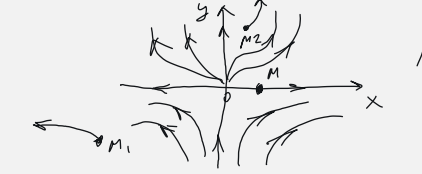
\includegraphics[width=0.75\textwidth]{figures/prklad_3_phase_portrait.png}
  \caption{Фазовий портрет системи (Приклад~3): вироджена особлива точка $O(0,0)$ типу сідло-вузол.}
  \label{fig:prklad_3}
\end{figure}

---

\section*{Приклад 4}
\begin{gather*}
\begin{cases}
\dot{x} = \left(x + \frac{1}{3}\right)\left(\frac{1}{2}y - x\right) \\
\dot{y} = \left(y - \frac{4}{3}\right)(x + y)
\end{cases}
\end{gather*}

Стани рівноваги: $O(0,0)$, $A\left(-\frac{1}{3}, \frac{4}{3}\right)$, $B\left(-\frac{1}{3}, \frac{1}{3}\right)$, $C\left(\frac{2}{3}, \frac{4}{3}\right)$. \\
Точка $O(0,0)$ -- стійкий фокус.

Побудуємо ізокліни:
\begin{itemize}
    \item Вертикальних нахилів ($\dot{x} = 0$): пряма $y = 2x$.
    \item Горизонтальних нахилів ($\dot{y} = 0$): пряма $y = -x$.
\end{itemize}

\begin{figure}[htbp]
  \centering
  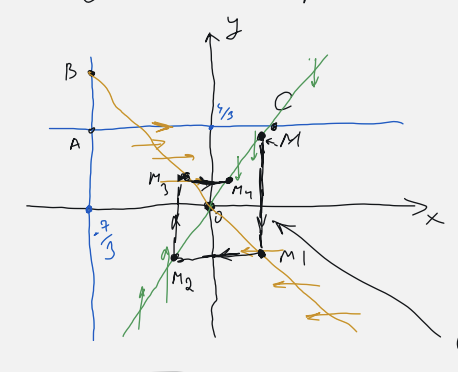
\includegraphics[width=0.85\textwidth]{figures/prklad_4_bez_kontaktiv.png}
  \caption{Метод ``без контактів'' (Приклад~4): ізокліни $y = 2x$ та $y = -x$, ламана $M \to M_1 \to M_2 \to M_3 \to M_4 \dots$ навколо стійкого фокуса $O(0,0)$.}
  \label{fig:prklad_4}
\end{figure}

За допомогою побудови відрізків ``без контактів'' (див. Малюнок~\ref{fig:prklad_4}) видно, що траєкторії, які виходять з точки $M$, роблять оберт навколо $O(0,0)$, наближаючись до центру, але ніколи не повертаються в початкову точку $M$. Це доводить відсутність періодичних розв'язків (замкнених граничних циклів) у цій області.

---

\section*{Приклад 5. Дослідження наявності періодичних розв'язків}
\begin{gather*}
\begin{cases}
\dot{x} = P(x,y) = y \\
\dot{y} = Q(x,y) = -(1 + x^2 + x^4)y - x
\end{cases}
\end{gather*}

Стан рівноваги $O(0,0)$ -- стійкий фокус. \\
Застосуємо \textbf{Критерій Бендіксона}:
$$\frac{\partial P(x,y)}{\partial x} + \frac{\partial Q(x,y)}{\partial y} = 0 - (1 + x^2 + x^4) = -(1 + x^2 + x^4) < 0 \quad (\forall (x,y) \in \mathbb{R}^2)$$

Оскільки дивергенція векторного поля зберігає сталий знак (строго менша за нуль) у всій площині, система \textbf{не має періодичних розв'язків (замкнених траєкторій)}.

---

\section*{Приклад 6. Дослідження граничних циклів}
\begin{gather*}
\begin{cases}
\dot{x} = y + x(x^2 + y^2 + 1) \\
\dot{y} = -x + y(x^2 + y^2 + 1)
\end{cases}
\end{gather*}

Дослідимо топологічну структуру за допомогою допоміжного сімейства концентричних кіл:
$$x^2 + y^2 = C$$

Знайдемо похідну вздовж траєкторій системи диференціальних рівнянь:
\begin{align*}
\frac{d}{dt}(x^2 + y^2) &= 2x\dot{x} + 2y\dot{y} \\
&= 2x[y + x(x^2 + y^2 + 1)] + 2y[-x + y(x^2 + y^2 + 1)] \\
&= 2xy + 2x^2(x^2 + y^2 + 1) - 2xy + 2y^2(x^2 + y^2 + 1) \\
&= 2(x^2 + y^2)(x^2 + y^2 + 1) \ge 0 \quad (\forall (x,y) \in \mathbb{R}^2)
\end{align*}

Оскільки похідна $\frac{d}{dt}(x^2+y^2) > 0$ у будь-якій точці площини, крім початку координат, кола $x^2 + y^2 = C$ утворюють сімейство замкнених кривих без контактів. Вздовж будь-якої траєкторії відстань від початку координат монотонно зростає з часом $t$, тому система \textbf{не має періодичних траєкторій (граничних циклів)}.

---

\section*{Приклад 7}
\begin{gather*}
\begin{cases}
\dot{x} = y \\
\dot{y} = 2(1 - x^2)y
\end{cases}
\end{gather*}

Дана система не має ізольованих станів рівноваги (всі особливі точки лежать на лінії $y=0$). Оскільки всередині будь-якої замкненої періодичної траєкторії (граничного циклу) обов'язково повинен міститися принаймні один ізольований стан рівноваги, дана система \textbf{не має періодичних траєкторій}.

\end{document}
